\documentclass[a4paper,10pt]{article}
\usepackage[hidelinks]{hyperref}
\usepackage{float}
\usepackage{graphicx}
\usepackage{listings}
\usepackage[utf8]{inputenc}
\usepackage{changepage}
\usepackage{etoolbox}
\usepackage{geometry}
\usepackage{booktabs}
\usepackage{longtable}
\renewcommand*\contentsname{Indice}

\makeatletter
\patchcmd\l@section{%
  \nobreak\hfil\nobreak
}{%
  \nobreak
  \leaders\hbox{%
    $\m@th \mkern \@dotsep mu\hbox{.}\mkern \@dotsep mu$%
  }%
  \hfill
  \nobreak
}{}{\errmessage{\noexpand\l@section could not be patched}}
\makeatother

\setcounter{secnumdepth}{0}

\begin{document}

\begin{titlepage}
\noindent
    \vspace*{5mm}
	\begin{minipage}[t]{0.15\textwidth}
	    \vspace*{5mm}
		\vspace{-3.5mm}{\includegraphics{img/logo_bicocca.png}}
	\end{minipage}
	\hspace{1cm}
	\begin{minipage}[t]{0.90\textwidth}
	      \vspace*{5mm}
		{
			{\textsc{Università degli Studi di Milano - Bicocca} } \\
			\textbf{Scuola di Scienze} \\
			\textbf{Dipartimento di Informatica, Sistemistica e Comunicazione} \\
			\textbf{Corso di Laurea Magistrale in Informatica} \\
			\par
		}
	\end{minipage}
	
	\vspace{42mm}

\begin{center}
    {\LARGE{
    
            \textbf{Multiple Sequence Alignment (MSA) di sequenze SARS-Cov2 \\ }
    }}        
\end{center}

\vspace{40mm}
	
	
	\begin{flushright}
		\large{Alberici Federico - 808058\\} 
		\large{Bettini Ivo Junior - 806878\\} 
		\large{Traversa Silvia - 816435} 
	\end{flushright}
	
	\vspace{15mm}
	\begin{center}
		{\large{\bf Anno Accademico 2019 - 2020}}
	\end{center}


\end{titlepage}

\tableofcontents

\newpage

\section{SARS-CoV-2}
I coronavirus sono una famiglia di virus RNA a filamento positivo con aspetto simile a una corona se esaminati al microscopio elettronico (da cui il nome) e noti per causare malattie che vanno dal comune raffreddore a patologie più gravi come la Sindrome respiratoria mediorientale (MERS) o la Sindrome respiratoria acuta grave (SARS). \\
Nel Dicembre 2019 a Wuhan, in Cina, è stato isolato un nuovo ceppo di coronavirus, denominato SARS-CoV-2 (\textit{Severe Acute Respiratory Syndrome - Coronavirus - 2}), la cui sequenza virale ha un'omologia del 76\% con il virus che causò la pandemia della Sars nel 2002.La malattia respiratoria causata da questo nuovo coronavirus è stata chiamata COVID-19.

\begin{figure}[H]
\centering
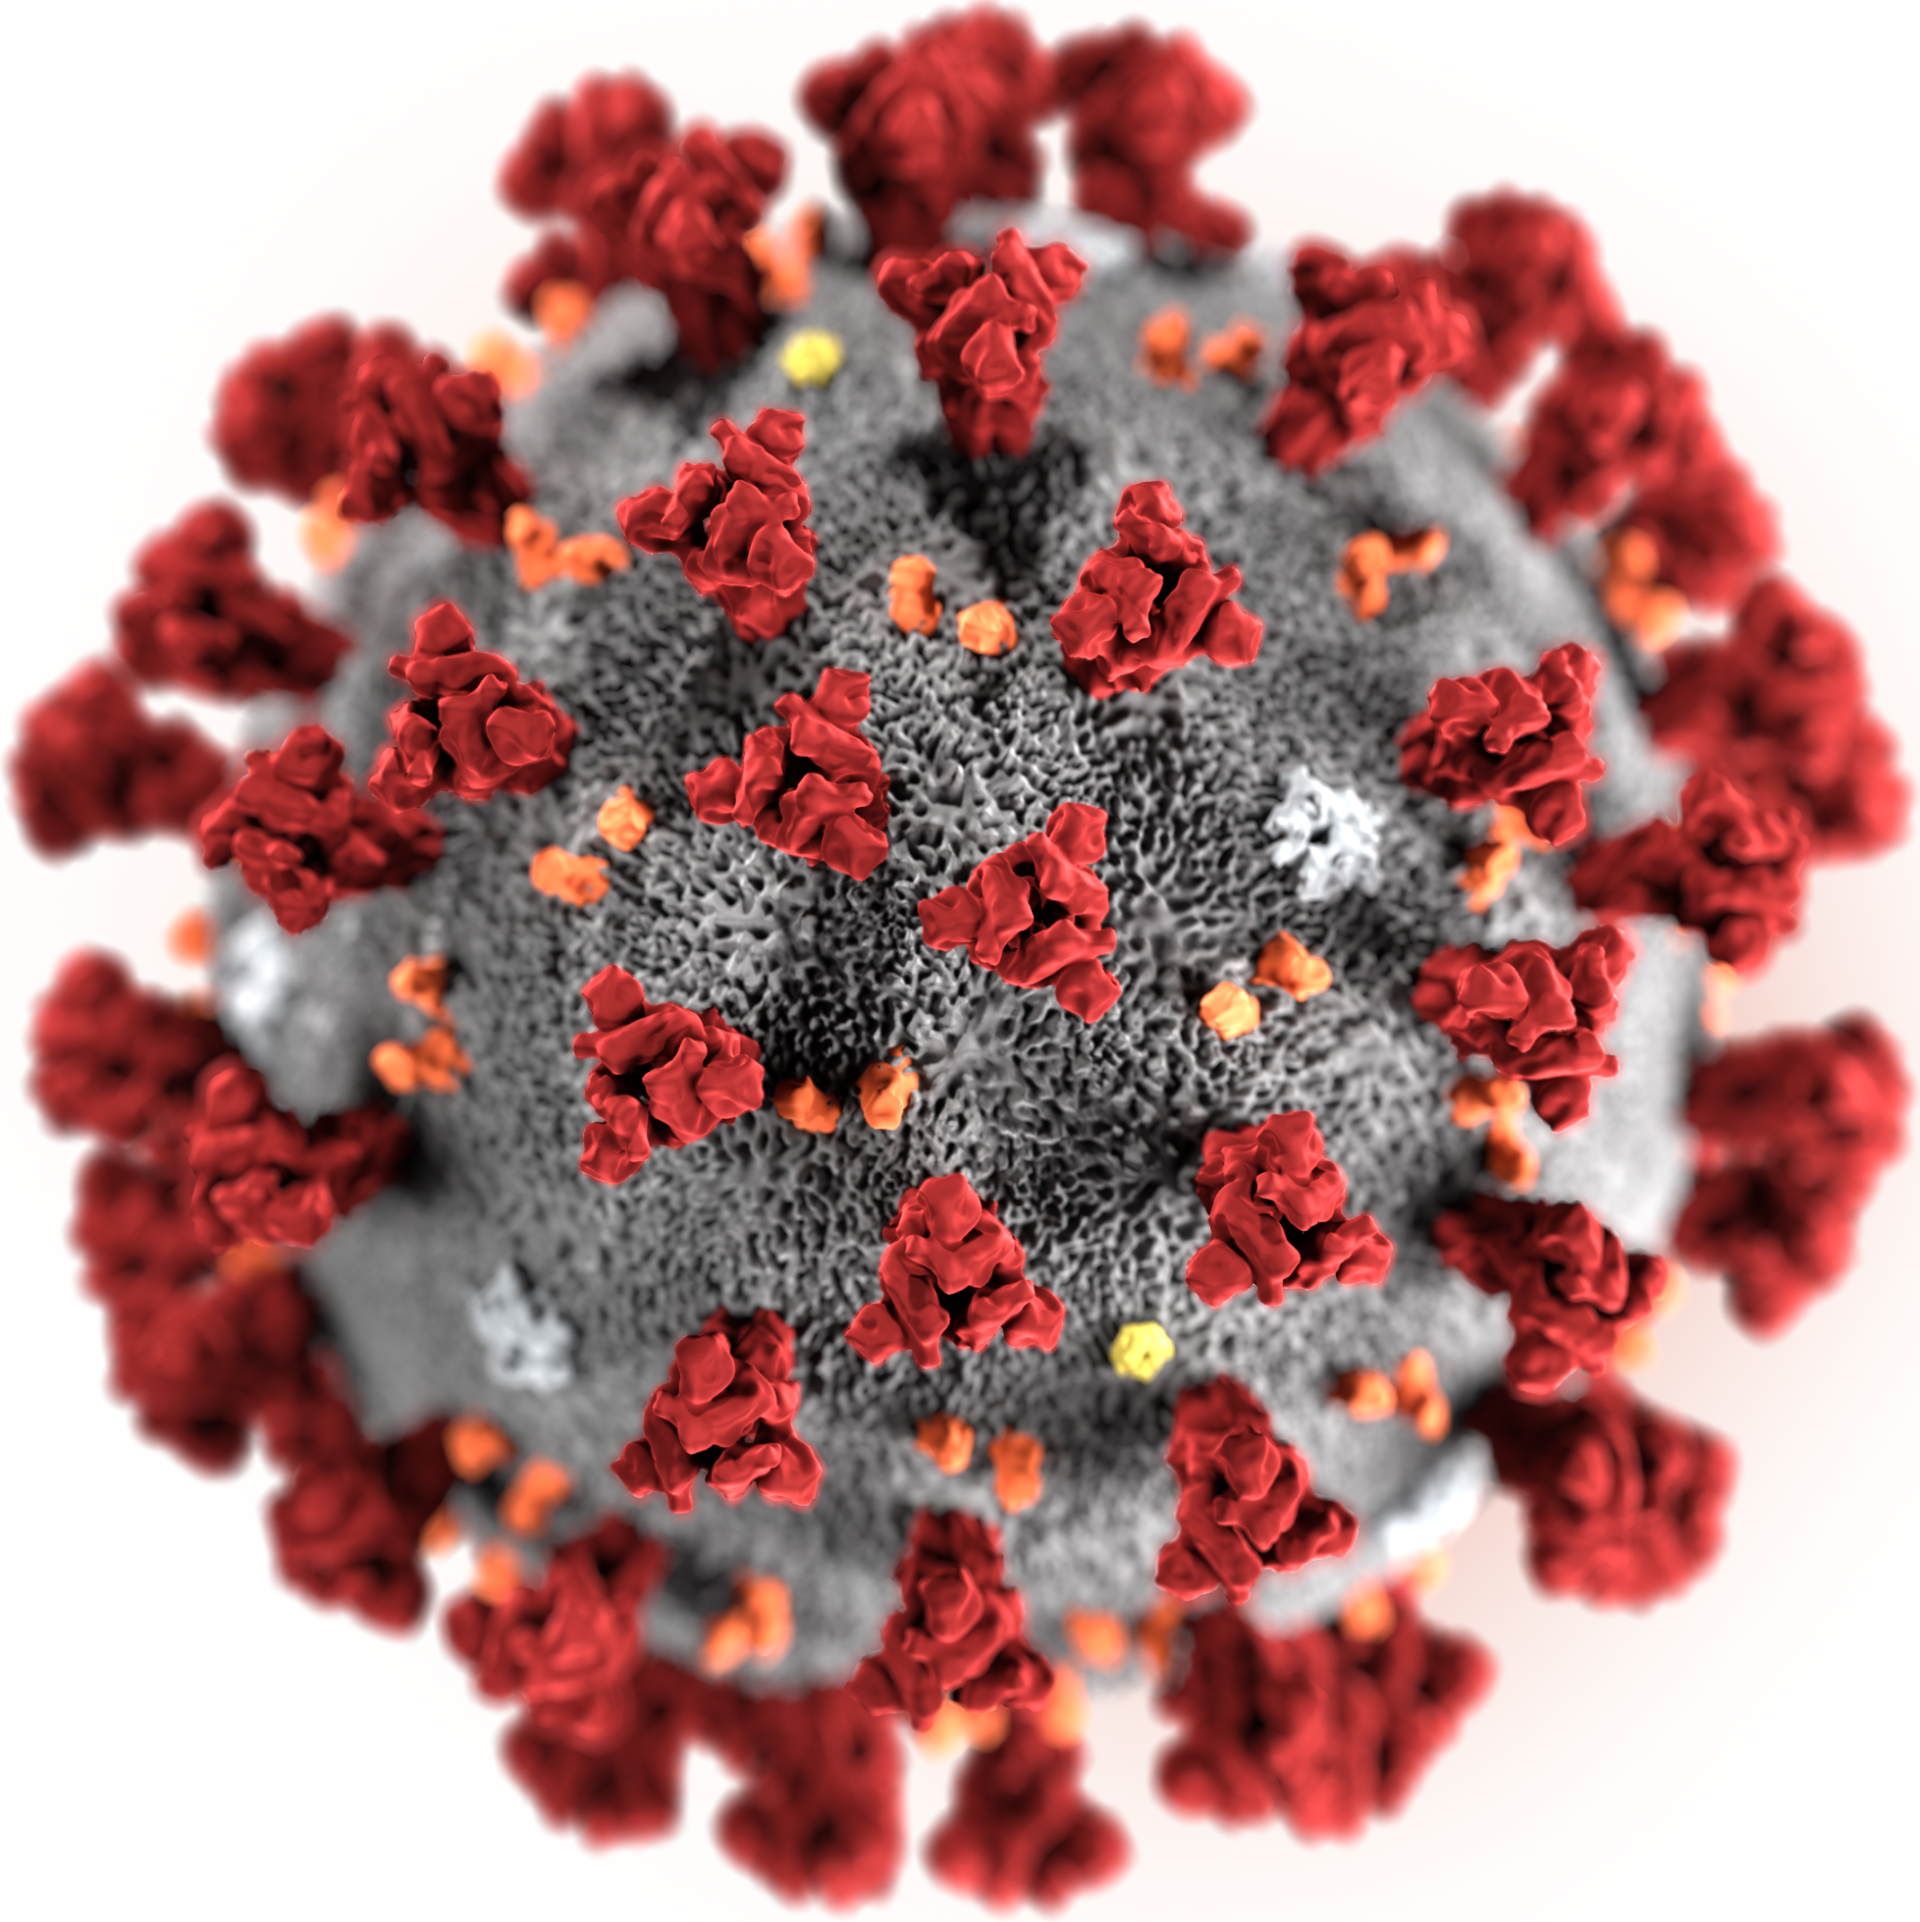
\includegraphics[width=.3\linewidth]{img/nCov.png}
\caption{\textit{L’illustrazione, creata dai Centers for Disease Control and Prevention (CDC) statunitense, rivela la morfologia ultrastrutturale del SARS-CoV-2}}
\label{fig:1}
\end{figure}

Ogni virione (singola particella virale) SARS-CoV-2 ha un diametro di circa 50-200 nanometri. Come altri coronavirus, SARS-CoV-2 presenta quattro proteine strutturali: S (spike), E (inviluppo), M (membrana) e N (nucleocapside). La proteina N contiene il genoma dell'RNA mentre le proteine S, E, M creano insieme l'inviluppo virale. %chiedere a prof Cattin
In particolare la proteina spike è quella che permette al virus di attaccarsi alla membrana di una cellula ospite.\\

Fra le sequenze genomiche SARS-CoV-2 note è stata evidenziata una bassa variabilità, si ritiene dunque che il ceppo sia stato rilevato dalle autorità sanitarie entro poche settimane dalla sua comparsa tra la popolazione umana alla fine del 2019.
Dopo il primo caso di infezione noto, avvenuto in Cina verso la fine del 2019, il virus si è diffuso in tutte le province della Cina e in oltre 150 altri paesi in Asia, Europa, Nord America, Sud America, Africa e Oceania.
La trasmissione da uomo a uomo di SARS-CoV-2 è stata confermata nel gennaio 2020 e avviene principalmente attraverso goccioline respiratorie da tosse e starnuti entro un raggio di circa 1,8 metri oppure un'altra possibile causa di infezione è il contatto indiretto tramite superfici contaminate.\\
Il numero di riproduzione di base del virus è stato stimato tra 1.4 e 3.9, il che significa che ogni infezione dal virus dovrebbe causare da 1.4 a 3.9 nuove infezioni nel caso in cui nessun membro della comunità sia immune e non vengano prese misure preventive.\\
Al 25 maggio 2020, ci sono stati 5.428.605 casi confermati totali di infezione da SARS-CoV-2 nella pandemia in corso, con un totale di decessi attribuiti al virus di 345.375. 

\newpage

\section{Obiettivo del progetto}
L'obiettivo del nostro progetto è riuscire ad allineare le sequenze scaricate (compresa quella che utlizziamo come riferimento per i confronti) con i tool scelti, e produrre in output le variazioni delle sequenze scaricate rispetto alla sequenza di riferimento e creare un'apposita documentazione. \\
Per poter raggiungere questo obiettivo, abbiamo deciso di dividere la nostra analisi in due parti:\\ 
\begin{itemize}
\item nella prima parte eseguiamo un'analisi verticale fra la sequenza di riferimento (ossia la prima sequenza che presente nella banca dati raccolta a Wuhan) e delle sequenze prese rispettivamente da Italia, New York, Spagna e Russia. Le sequenze dei singoli paesi sono state prese seguendo un ordine temporale crescente, in modo tale da poter denotare attraverso il confronto delle mutazioni nel tempo.
\item nella seconda parte, invece, effettuiamo un confronto orizzontale tra le ultime sequenze raccolte dei vari paesi scelti, in modo da poter individuare la presenza di eventuali mutazioni nello stato corrente del virus, sempre tenedo come riferimanto la prima sequenze presente nella banca dati. 
\end{itemize}

\section{Sequenze}
Abbiamo deciso di selezionare alcuni dei paesi con il più alto numero di casi di COVID-19, ossia Stati Uniti (per il quale ci siamo concentrati su uno degli stati a sua volta più colpito, quello di New York), Russia,  Spagna e Italia. I casi, al 25 Maggio 2020, sono riportati nella tabella seguente:

\begin{table}[H]
\centering
\begin{tabular}{|l|l|}
\hline
\textbf{Stati Uniti} & 1,678,477 \\ \hline
\textbf{Russia}      & 353,427   \\ \hline
\textbf{Spagna}      & 235,823   \\ \hline
\textbf{Italia}      & 229,858   \\ \hline
\end{tabular}
\end{table}

Le sequenze analizzate sono state prese dal sito GISAID. Per ogni paese abbiamo preso solo sequenze complete (con più di 29000 basi) e su pazienti tutti di sesso maschile. Abbiamo cercato inoltre di seguire una linea temporale che partisse dalla prima sequenza presente nel database fino all'ultima, con in mezzo sequenze che si distanziavano tra di loro di una settimana.

\section{Tool}
Tra i tool messi a disposizione abbiamo scelto di utilizzare Clustal Omega, Kalign e MAFFT.\\
Abbiamo scelto Clustal Omega poichè sfrutta il modello probabilistico Profilo HMM (Hidden Markov Model), il quale è in grado di incapsulare i cambiamenti evolutivi che si sono verificati in una serie di sequenze correlate ed inoltre questo tool risultava ottimale per sequenze molto lunghe.\\
Kalign è stato scelto poichè è un tool che si concentra sulle regioni locali e lavora molto velocemente, motivo per il quale ci sembrava particolarmente adatto per le analisi sui singoli stati che volevamo svolgere.\\
Infine abbiamo scelto MAFFT poichè attraverso l'algoritmo della trasformata di Fourier veloce ottimizza gli allineamenti in base alle proprietà fisiche, utilizzando sia un allineamento progressivo che iterativo. Anche esso risulta essere ottimale per sequenze di lunghezza medio-grandi.

\section{Analisi verticale}

\subsection{New York (USA)}

\subsection{Russia}

\subsection{Italia}


\subsection{Spagna}
%Dobbiamo allegare in qualche modo il file di output ottenuto. Più ovviamento un commento sul risultato

\newpage

\section{Appendice A - risultati estesi}

\newpage

\newgeometry{left=0.5cm, top=0.3cm}
\subsection{Italia}

\subsubsection{Clustal Omega}

% Please add the following required packages to your document preamble:
% \usepackage{booktabs}
% \usepackage{longtable}
% Note: It may be necessary to compile the document several times to get a multi-page table to line up properly
\begin{longtable}{@{}ccccc@{}}


\toprule
\textbf{ID\_SEQ} & \textbf{POS} & \textbf{LENGTH} & \textbf{REFERENCE} & \textbf{MUTATION} \\* \midrule
\endfirsthead
%
\cline{1-5}
\endhead
%
1\_Italy|EPI\_ISL\_412974 & 11083 & 1 & G & T \\* \midrule
1\_Italy|EPI\_ISL\_412974 & 26144 & 1 & G & T \\* \midrule
2\_Italy|EPI\_ISL\_412973 & 241 & 1 & C & T \\* \midrule
2\_Italy|EPI\_ISL\_412973 & 3037 & 1 & C & T \\* \midrule
2\_Italy|EPI\_ISL\_412973 & 14408 & 1 & C & T \\* \midrule
2\_Italy|EPI\_ISL\_412973 & 23403 & 1 & A & G \\* \midrule
2\_Italy|EPI\_ISL\_412973 & 29867 & 2 & TG & NN \\* \midrule
3\_Italy|EPI\_ISL\_417423 & 0 & 1 & - & G \\* \midrule
3\_Italy|EPI\_ISL\_417423 & 241 & 1 & C & T \\* \midrule
3\_Italy|EPI\_ISL\_417423 & 3037 & 1 & C & T \\* \midrule
3\_Italy|EPI\_ISL\_417423 & 14408 & 1 & C & T \\* \midrule
3\_Italy|EPI\_ISL\_417423 & 23403 & 1 & A & G \\* \midrule
3\_Italy|EPI\_ISL\_417423 & 29891 & 13 & AAAAAAAAAAAAA & ------------- \\* \midrule
4\_Italy|EPI\_ISL\_418256 & 42 & 1 & T & Y \\* \midrule
4\_Italy|EPI\_ISL\_418256 & 44 & 2 & CG & NN \\* \midrule
4\_Italy|EPI\_ISL\_418256 & 241 & 1 & C & T \\* \midrule
4\_Italy|EPI\_ISL\_418256 & 3037 & 1 & C & T \\* \midrule
4\_Italy|EPI\_ISL\_418256 & 14408 & 1 & C & T \\* \midrule
4\_Italy|EPI\_ISL\_418256 & 23403 & 1 & A & G \\* \midrule
4\_Italy|EPI\_ISL\_418256 & 28881 & 3 & GGG & AAC \\* \midrule
4\_Italy|EPI\_ISL\_418256 & 29899 & 5 & AAAAA & ----- \\* \midrule
5\_Italy|EPI\_ISL\_419254 & 1 & 25 & ATTAAAGGTTTATACCTTCCCAGGT & ------------------------- \\* \midrule
5\_Italy|EPI\_ISL\_419254 & 241 & 1 & C & T \\* \midrule
5\_Italy|EPI\_ISL\_419254 & 3037 & 1 & C & T \\* \midrule
5\_Italy|EPI\_ISL\_419254 & 14408 & 1 & C & T \\* \midrule
5\_Italy|EPI\_ISL\_419254 & 23403 & 1 & A & G \\* \midrule
5\_Italy|EPI\_ISL\_419254 & 29860 & 44 & \begin{tabular}[c]{@{}c@{}}AGGAGAATGACAAAAAAAAAA\\ AAAAAAAAAAAAAAAAAAAAAAA\end{tabular} & \begin{tabular}[c]{@{}c@{}}-----------------------\\ ---------------------\end{tabular} \\* \midrule
6\_Italy|EPI\_ISL\_428854 & 241 & 1 & C & T \\* \midrule
6\_Italy|EPI\_ISL\_428854 & 3037 & 1 & C & T \\* \midrule
6\_Italy|EPI\_ISL\_428854 & 14408 & 1 & C & T \\* \midrule
6\_Italy|EPI\_ISL\_428854 & 23403 & 1 & A & G \\* \midrule
6\_Italy|EPI\_ISL\_428854 & 29009 & 1 & G & A \\* \midrule
6\_Italy|EPI\_ISL\_428854 & 29900 & 4 & AAAA & ---- \\* \midrule
7\_Italy|EPI\_ISL\_435152 & 1 & 37 & \begin{tabular}[c]{@{}c@{}}ATTAAAGGTTTATACCTTCC\\ CAGGTAACAAACCAACC\end{tabular} & \begin{tabular}[c]{@{}c@{}}NNNNNNNNNNNNNNNNNNN\\ NNNNNNNNNNNNNNNNNN\end{tabular} \\* \midrule
7\_Italy|EPI\_ISL\_435152 & 241 & 1 & C & T \\* \midrule
7\_Italy|EPI\_ISL\_435152 & 3037 & 1 & C & T \\* \midrule
7\_Italy|EPI\_ISL\_435152 & 5986 & 1 & C & T \\* \midrule
7\_Italy|EPI\_ISL\_435152 & 6866 & 1 & A & W \\* \midrule
7\_Italy|EPI\_ISL\_435152 & 6869 & 1 & A & W \\* \midrule
7\_Italy|EPI\_ISL\_435152 & 14408 & 1 & C & T \\* \midrule
7\_Italy|EPI\_ISL\_435152 & 23403 & 1 & A & G \\* \midrule
7\_Italy|EPI\_ISL\_435152 & 28881 & 3 & GGG & AAC \\* \midrule
7\_Italy|EPI\_ISL\_435152 & 29701 & 1 & G & T \\* \midrule
7\_Italy|EPI\_ISL\_435152 & 29879 & 25 & \begin{tabular}[c]{@{}c@{}}AAAAAAAAAAAAA\\ AAAAAAAAAAAA\end{tabular} & \begin{tabular}[c]{@{}c@{}}--------------\\ -----------\end{tabular} \\* \midrule
8\_Italy|EPI\_ISL\_436729 & 1 & 9 & ATTAAAGGT & NNNNNNNNN \\* \midrule
8\_Italy|EPI\_ISL\_436729 & 31 & 1 & A & G \\* \midrule
8\_Italy|EPI\_ISL\_436729 & 241 & 1 & C & T \\* \midrule
8\_Italy|EPI\_ISL\_436729 & 3037 & 1 & C & T \\* \midrule
8\_Italy|EPI\_ISL\_436729 & 3045 & 1 & C & T \\* \midrule
8\_Italy|EPI\_ISL\_436729 & 6449 & 1 & C & T \\* \midrule
8\_Italy|EPI\_ISL\_436729 & 6863 & 1 & A & M \\* \midrule
8\_Italy|EPI\_ISL\_436729 & 6866 & 1 & A & W \\* \midrule
8\_Italy|EPI\_ISL\_436729 & 6869 & 1 & A & W \\* \midrule
8\_Italy|EPI\_ISL\_436729 & 14408 & 1 & C & T \\* \midrule
8\_Italy|EPI\_ISL\_436729 & 19677 & 1 & G & R \\* \midrule
8\_Italy|EPI\_ISL\_436729 & 21627 & 1 & C & Y \\* \midrule
8\_Italy|EPI\_ISL\_436729 & 23403 & 1 & A & G \\* \midrule
8\_Italy|EPI\_ISL\_436729 & 25459 & 1 & G & K \\* \midrule
8\_Italy|EPI\_ISL\_436729 & 28881 & 3 & GGG & AAC \\* \midrule
8\_Italy|EPI\_ISL\_436729 & 29874 & 30 & \begin{tabular}[c]{@{}c@{}}AAAAAAAAAAAAAAA\\ AAAAAAAAAAAAAAA\end{tabular} & \begin{tabular}[c]{@{}c@{}}----------------\\ --------------\end{tabular} \\* \bottomrule
\end{longtable}

\newpage
\subsubsection{Kalign}

% Please add the following required packages to your document preamble:
% \usepackage{booktabs}
% \usepackage{longtable}
% Note: It may be necessary to compile the document several times to get a multi-page table to line up properly
\begin{longtable}{@{}ccccc@{}}
\toprule
\textbf{ID\_SEQ} & \textbf{POS} & \textbf{LENGTH} & \textbf{REFERENCE} & \textbf{MUTATION} \\* \midrule
\endfirsthead
%
\cline{1-5}
\endhead
%
1\_Italy|EPI\_ISL\_412974 & 11083 & 1 & G & T \\* \midrule
1\_Italy|EPI\_ISL\_412974 & 26144 & 1 & G & T \\* \midrule
2\_Italy|EPI\_ISL\_412973 & 241 & 1 & C & T \\* \midrule
2\_Italy|EPI\_ISL\_412973 & 3037 & 1 & C & T \\* \midrule
2\_Italy|EPI\_ISL\_412973 & 14408 & 1 & C & T \\* \midrule
2\_Italy|EPI\_ISL\_412973 & 23403 & 1 & A & G \\* \midrule
2\_Italy|EPI\_ISL\_412973 & 29867 & 2 & TG & NN \\* \midrule
3\_Italy|EPI\_ISL\_417423 & 0 & 1 & - & G \\* \midrule
3\_Italy|EPI\_ISL\_417423 & 241 & 1 & C & T \\* \midrule
3\_Italy|EPI\_ISL\_417423 & 3037 & 1 & C & T \\* \midrule
3\_Italy|EPI\_ISL\_417423 & 14408 & 1 & C & T \\* \midrule
3\_Italy|EPI\_ISL\_417423 & 23403 & 1 & A & G \\* \midrule
3\_Italy|EPI\_ISL\_417423 & 29879 & 13 & AAAAAAAAAAAAA & ------------- \\* \midrule
4\_Italy|EPI\_ISL\_418256 & 42 & 1 & T & Y \\* \midrule
4\_Italy|EPI\_ISL\_418256 & 44 & 2 & CG & NN \\* \midrule
4\_Italy|EPI\_ISL\_418256 & 241 & 1 & C & T \\* \midrule
4\_Italy|EPI\_ISL\_418256 & 3037 & 1 & C & T \\* \midrule
4\_Italy|EPI\_ISL\_418256 & 14408 & 1 & C & T \\* \midrule
4\_Italy|EPI\_ISL\_418256 & 23403 & 1 & A & G \\* \midrule
4\_Italy|EPI\_ISL\_418256 & 28881 & 3 & GGG & AAC \\* \midrule
4\_Italy|EPI\_ISL\_418256 & 29879 & 5 & AAAAA & ----- \\* \midrule
5\_Italy|EPI\_ISL\_419254 & 1 & 25 & \begin{tabular}[c]{@{}c@{}}ATTAAAGGTTTAT\\ ACCTTCCCAGGT\end{tabular} & ------------------------- \\* \midrule
5\_Italy|EPI\_ISL\_419254 & 241 & 1 & C & T \\* \midrule
5\_Italy|EPI\_ISL\_419254 & 3037 & 1 & C & T \\* \midrule
5\_Italy|EPI\_ISL\_419254 & 14408 & 1 & C & T \\* \midrule
5\_Italy|EPI\_ISL\_419254 & 23403 & 1 & A & G \\* \midrule
5\_Italy|EPI\_ISL\_419254 & 29860 & 44 & \begin{tabular}[c]{@{}c@{}}AGGAGAATGACAAAAAAAAAA\\ AAAAAAAAAAAAAAAAAAAAAAA\end{tabular} & \begin{tabular}[c]{@{}c@{}}-----------------------\\ ---------------------\end{tabular} \\* \midrule
6\_Italy|EPI\_ISL\_428854 & 241 & 1 & C & T \\* \midrule
6\_Italy|EPI\_ISL\_428854 & 3037 & 1 & C & T \\* \midrule
6\_Italy|EPI\_ISL\_428854 & 14408 & 1 & C & T \\* \midrule
6\_Italy|EPI\_ISL\_428854 & 23403 & 1 & A & G \\* \midrule
6\_Italy|EPI\_ISL\_428854 & 29009 & 1 & G & A \\* \midrule
6\_Italy|EPI\_ISL\_428854 & 29879 & 4 & AAAA & ---- \\* \midrule
7\_Italy|EPI\_ISL\_435152 & 1 & 37 & \begin{tabular}[c]{@{}c@{}}ATTAAAGGTTTATACCTTC\\ CCAGGTAACAAACCAACC\end{tabular} & \begin{tabular}[c]{@{}c@{}}NNNNNNNNNNNNNNNNNN\\ NNNNNNNNNNNNNNNNNNN\end{tabular} \\* \midrule
7\_Italy|EPI\_ISL\_435152 & 241 & 1 & C & T \\* \midrule
7\_Italy|EPI\_ISL\_435152 & 3037 & 1 & C & T \\* \midrule
7\_Italy|EPI\_ISL\_435152 & 5986 & 1 & C & T \\* \midrule
7\_Italy|EPI\_ISL\_435152 & 6866 & 1 & A & W \\* \midrule
7\_Italy|EPI\_ISL\_435152 & 6869 & 1 & A & W \\* \midrule
7\_Italy|EPI\_ISL\_435152 & 14408 & 1 & C & T \\* \midrule
7\_Italy|EPI\_ISL\_435152 & 23403 & 1 & A & G \\* \midrule
7\_Italy|EPI\_ISL\_435152 & 28881 & 3 & GGG & AAC \\* \midrule
7\_Italy|EPI\_ISL\_435152 & 29701 & 1 & G & T \\* \midrule
7\_Italy|EPI\_ISL\_435152 & 29879 & 25 & \begin{tabular}[c]{@{}c@{}}AAAAAAAAAAAA\\ AAAAAAAAAAAAA\end{tabular} & ------------------------- \\* \midrule
8\_Italy|EPI\_ISL\_436729 & 1 & 9 & ATTAAAGGT & NNNNNNNNN \\* \midrule
8\_Italy|EPI\_ISL\_436729 & 31 & 1 & A & G \\* \midrule
8\_Italy|EPI\_ISL\_436729 & 241 & 1 & C & T \\* \midrule
8\_Italy|EPI\_ISL\_436729 & 3037 & 1 & C & T \\* \midrule
8\_Italy|EPI\_ISL\_436729 & 3045 & 1 & C & T \\* \midrule
8\_Italy|EPI\_ISL\_436729 & 6449 & 1 & C & T \\* \midrule
8\_Italy|EPI\_ISL\_436729 & 6863 & 1 & A & M \\* \midrule
8\_Italy|EPI\_ISL\_436729 & 6866 & 1 & A & W \\* \midrule
8\_Italy|EPI\_ISL\_436729 & 6869 & 1 & A & W \\* \midrule
8\_Italy|EPI\_ISL\_436729 & 14408 & 1 & C & T \\* \midrule
8\_Italy|EPI\_ISL\_436729 & 19677 & 1 & G & R \\* \midrule
8\_Italy|EPI\_ISL\_436729 & 21627 & 1 & C & Y \\* \midrule
8\_Italy|EPI\_ISL\_436729 & 23403 & 1 & A & G \\* \midrule
8\_Italy|EPI\_ISL\_436729 & 25459 & 1 & G & K \\* \midrule
8\_Italy|EPI\_ISL\_436729 & 28881 & 3 & GGG & AAC \\* \midrule
8\_Italy|EPI\_ISL\_436729 & 29874 & 30 & \begin{tabular}[c]{@{}c@{}}AAAAAAAAAAAAAAA\\ AAAAAAAAAAAAAAA\end{tabular} & ------------------------------ \\* \bottomrule
\end{longtable}

\newpage

\subsubsection{MAFFT}

% Please add the following required packages to your document preamble:
% \usepackage{booktabs}
% \usepackage{longtable}
% Note: It may be necessary to compile the document several times to get a multi-page table to line up properly
\begin{longtable}{@{}ccccc@{}}
\toprule
\textbf{ID\_SEQ} & \textbf{POS} & \textbf{LENGTH} & \textbf{REFERENCE} & \textbf{MUTATION} \\* \midrule
\endfirsthead
%
\cline{1-5}
\endhead
%
1\_Italy|EPI\_ISL\_412974 & 11083 & 1 & G & T \\* \midrule
1\_Italy|EPI\_ISL\_412974 & 26144 & 1 & G & T \\* \midrule
2\_Italy|EPI\_ISL\_412973 & 241 & 1 & C & T \\* \midrule
2\_Italy|EPI\_ISL\_412973 & 3037 & 1 & C & T \\* \midrule
2\_Italy|EPI\_ISL\_412973 & 14408 & 1 & C & T \\* \midrule
2\_Italy|EPI\_ISL\_412973 & 23403 & 1 & A & G \\* \midrule
2\_Italy|EPI\_ISL\_412973 & 29867 & 2 & TG & NN \\* \midrule
3\_Italy|EPI\_ISL\_417423 & 0 & 1 & - & G \\* \midrule
3\_Italy|EPI\_ISL\_417423 & 241 & 1 & C & T \\* \midrule
3\_Italy|EPI\_ISL\_417423 & 3037 & 1 & C & T \\* \midrule
3\_Italy|EPI\_ISL\_417423 & 14408 & 1 & C & T \\* \midrule
3\_Italy|EPI\_ISL\_417423 & 23403 & 1 & A & G \\* \midrule
3\_Italy|EPI\_ISL\_417423 & 29890 & 13 & AAAAAAAAAAAAA & ------------- \\* \midrule
4\_Italy|EPI\_ISL\_418256 & 42 & 1 & T & Y \\* \midrule
4\_Italy|EPI\_ISL\_418256 & 44 & 2 & CG & NN \\* \midrule
4\_Italy|EPI\_ISL\_418256 & 241 & 1 & C & T \\* \midrule
4\_Italy|EPI\_ISL\_418256 & 3037 & 1 & C & T \\* \midrule
4\_Italy|EPI\_ISL\_418256 & 14408 & 1 & C & T \\* \midrule
4\_Italy|EPI\_ISL\_418256 & 23403 & 1 & A & G \\* \midrule
4\_Italy|EPI\_ISL\_418256 & 28881 & 3 & GGG & AAC \\* \midrule
4\_Italy|EPI\_ISL\_418256 & 29898 & 5 & AAAAA & ----- \\* \midrule
5\_Italy|EPI\_ISL\_419254 & 1 & 25 & \begin{tabular}[c]{@{}c@{}}ATTAAAGGTTTATA\\ CCTTCCCAGGT\end{tabular} & ------------------------- \\* \midrule
5\_Italy|EPI\_ISL\_419254 & 241 & 1 & C & T \\* \midrule
5\_Italy|EPI\_ISL\_419254 & 3037 & 1 & C & T \\* \midrule
5\_Italy|EPI\_ISL\_419254 & 14408 & 1 & C & T \\* \midrule
5\_Italy|EPI\_ISL\_419254 & 23403 & 1 & A & G \\* \midrule
5\_Italy|EPI\_ISL\_419254 & 29859 & 44 & \begin{tabular}[c]{@{}c@{}}AGGAGAATGACAAAAAAAAAAA\\ AAAAAAAAAAAAAAAAAAAAAA\end{tabular} & -------------------------------------------- \\* \midrule
6\_Italy|EPI\_ISL\_428854 & 241 & 1 & C & T \\* \midrule
6\_Italy|EPI\_ISL\_428854 & 3037 & 1 & C & T \\* \midrule
6\_Italy|EPI\_ISL\_428854 & 14408 & 1 & C & T \\* \midrule
6\_Italy|EPI\_ISL\_428854 & 23403 & 1 & A & G \\* \midrule
6\_Italy|EPI\_ISL\_428854 & 29009 & 1 & G & A \\* \midrule
6\_Italy|EPI\_ISL\_428854 & 29899 & 4 & AAAA & ---- \\* \midrule
7\_Italy|EPI\_ISL\_435152 & 1 & 37 & \begin{tabular}[c]{@{}c@{}}ATTAAAGGTTTATACCTTCC\\ CAGGTAACAAACCAACC\end{tabular} & \begin{tabular}[c]{@{}c@{}}NNNNNNNNNNNNNNNNNN\\ NNNNNNNNNNNNNNNNNNN\end{tabular} \\* \midrule
7\_Italy|EPI\_ISL\_435152 & 241 & 1 & C & T \\* \midrule
7\_Italy|EPI\_ISL\_435152 & 3037 & 1 & C & T \\* \midrule
7\_Italy|EPI\_ISL\_435152 & 5986 & 1 & C & T \\* \midrule
7\_Italy|EPI\_ISL\_435152 & 6866 & 1 & A & W \\* \midrule
7\_Italy|EPI\_ISL\_435152 & 6869 & 1 & A & W \\* \midrule
7\_Italy|EPI\_ISL\_435152 & 14408 & 1 & C & T \\* \midrule
7\_Italy|EPI\_ISL\_435152 & 23403 & 1 & A & G \\* \midrule
7\_Italy|EPI\_ISL\_435152 & 28881 & 3 & GGG & AAC \\* \midrule
7\_Italy|EPI\_ISL\_435152 & 29701 & 1 & G & T \\* \midrule
7\_Italy|EPI\_ISL\_435152 & 29878 & 25 & \begin{tabular}[c]{@{}c@{}}AAAAAAAAAAAA\\ AAAAAAAAAAAAA\end{tabular} & ------------------------- \\* \midrule
8\_Italy|EPI\_ISL\_436729 & 1 & 9 & ATTAAAGGT & NNNNNNNNN \\* \midrule
8\_Italy|EPI\_ISL\_436729 & 31 & 1 & A & G \\* \midrule
8\_Italy|EPI\_ISL\_436729 & 241 & 1 & C & T \\* \midrule
8\_Italy|EPI\_ISL\_436729 & 3037 & 1 & C & T \\* \midrule
8\_Italy|EPI\_ISL\_436729 & 3045 & 1 & C & T \\* \midrule
8\_Italy|EPI\_ISL\_436729 & 6449 & 1 & C & T \\* \midrule
8\_Italy|EPI\_ISL\_436729 & 6863 & 1 & A & M \\* \midrule
8\_Italy|EPI\_ISL\_436729 & 6866 & 1 & A & W \\* \midrule
8\_Italy|EPI\_ISL\_436729 & 6869 & 1 & A & W \\* \midrule
8\_Italy|EPI\_ISL\_436729 & 14408 & 1 & C & T \\* \midrule
8\_Italy|EPI\_ISL\_436729 & 19677 & 1 & G & R \\* \midrule
8\_Italy|EPI\_ISL\_436729 & 21627 & 1 & C & Y \\* \midrule
8\_Italy|EPI\_ISL\_436729 & 23403 & 1 & A & G \\* \midrule
8\_Italy|EPI\_ISL\_436729 & 25459 & 1 & G & K \\* \midrule
8\_Italy|EPI\_ISL\_436729 & 28881 & 3 & GGG & AAC \\* \midrule
8\_Italy|EPI\_ISL\_436729 & 29873 & 30 & \begin{tabular}[c]{@{}c@{}}AAAAAAAAAAAAAAAA\\ AAAAAAAAAAAAAA\end{tabular} & ------------------------------ \\* \bottomrule
\end{longtable}

\newpage

\subsection{Spagna}

\subsubsection{Clustal Omega}

% Please add the following required packages to your document preamble:
% \usepackage{booktabs}
% \usepackage{longtable}
% Note: It may be necessary to compile the document several times to get a multi-page table to line up properly
\begin{longtable}{@{}ccccc@{}}
\toprule
\textbf{ID\_SEQ} & \textbf{POS} & \textbf{LENGTH} & \textbf{REFERENCE} & \textbf{MUTATION} \\* \midrule
\endfirsthead
%
\cline{1-5}
\endhead
%
1\_Spain|EPI\_ISL\_418251 & 240 & 1 & C & T \\* \midrule
1\_Spain|EPI\_ISL\_418251 & 3036 & 1 & C & T \\* \midrule
1\_Spain|EPI\_ISL\_418251 & 8781 & 1 & C & T \\* \midrule
1\_Spain|EPI\_ISL\_418251 & 11243 & 1 & T & C \\* \midrule
1\_Spain|EPI\_ISL\_418251 & 14407 & 1 & C & T \\* \midrule
1\_Spain|EPI\_ISL\_418251 & 21262 & 1 & C & T \\* \midrule
1\_Spain|EPI\_ISL\_418251 & 23402 & 1 & A & G \\* \midrule
1\_Spain|EPI\_ISL\_418251 & 29780 & 122 & \begin{tabular}[c]{@{}c@{}}AGCTGCCTATATGGAAGAGC\\ CCTAATGTGTAAAATTAATT\\ TTAGTAGTGCTATCCCCATG\\ TGATTTTAATAGCTTCTTAG\\ GAGAATGACAAAAAAAAAAA\\ AAAAAAAAAAAAAAAAAAAA\\ AA\end{tabular} & \begin{tabular}[c]{@{}c@{}}--------------------\\ ---------------------\\ ---------------------\\ ---------------------\\ ---------------------\\ ------------------\end{tabular} \\* \midrule
2\_Spain|EPI\_ISL\_419240 & 8781 & 1 & C & T \\* \midrule
2\_Spain|EPI\_ISL\_419240 & 9476 & 1 & T & A \\* \midrule
2\_Spain|EPI\_ISL\_419240 & 14804 & 1 & C & T \\* \midrule
2\_Spain|EPI\_ISL\_419240 & 25978 & 1 & G & T \\* \midrule
2\_Spain|EPI\_ISL\_419240 & 28143 & 1 & T & C \\* \midrule
2\_Spain|EPI\_ISL\_419240 & 28656 & 1 & C & T \\* \midrule
2\_Spain|EPI\_ISL\_419240 & 28862 & 1 & C & T \\* \midrule
2\_Spain|EPI\_ISL\_419240 & 29786 & 116 & \begin{tabular}[c]{@{}c@{}}CTATATGGAAGAGCCCTAATG\\ TGTAAAATTAATTTTAGTAGTG\\ CTATCCCCATGTGATTTTAATA\\ GCTTCTTAGGAGAATGACAA\\ AAAAAAAAAAAAAAAAAAA\\ AAAAAAAAAAAA\end{tabular} & \begin{tabular}[c]{@{}c@{}}--------------------\\ --------------------\\ --------------------\\ --------------------\\ --------------------\\ ----------------\end{tabular} \\* \midrule
3\_Spain|EPI\_ISL\_419685 & 0 & 54 & \begin{tabular}[c]{@{}c@{}}ATTAAAGGTTTATACCTTCCC\\ AGGTAACAAACCAACCAACT\\ TTCGATCTCTTGT\end{tabular} & \begin{tabular}[c]{@{}c@{}}--------------------\\ ---------------------\\ -------------\end{tabular} \\* \midrule
3\_Spain|EPI\_ISL\_419685 & 2000 & 1 & G & A \\* \midrule
3\_Spain|EPI\_ISL\_419685 & 5296 & 290 & \begin{tabular}[c]{@{}c@{}}ACTGCATTGTTAACACTCCA\\ ACAAATAGAGTTGAAGTTTA\\ ATCCACCTGCTCTACAAGAT\\ GCTTATTACAGAGCAAGGGC\\ TGGTGAAGCTGCTAACTTTT\\ GTGCACTTATCTTAGCCTAC\\ TGTAATAAGACAGTAGGTGA\\ GTTAGGTGATGTTAGAGAAA\\ CAATGAGTTACTTGTTTCAA\\ CATGCCAATTTAGATTCTTG\\ CAAAAGAGTCTTGAACGTGG\\ TGTGTAAAACTTGTGGACAA\\ CAGCAGACAACCCTTAAGGG\\ TGTAGAAGCTGTTATGTACA\\ TGGGCACACT\end{tabular} & \begin{tabular}[c]{@{}c@{}}NNNNNNNNNNNNNNNNNNNNN\\ NNNNNNNNNNNNNNNNNNNNN\\ NNNNNNNNNNNNNNNNNNNNN\\ NNNNNNNNNNNNNNNNNNNNN\\ NNNNNNNNNNNNNNNNNNNNN\\ NNNNNNNNNNNNNNNNNNNNN\\ NNNNNNNNNNNNNNNNNNNNN\\ NNNNNNNNNNNNNNNNNNNNN\\ NNNNNNNNNNNNNNNNNNNNN\\ NNNNNNNNNNNNNNNNNNNNN\\ NNNNNNNNNNNNNNNNNNNNN\\ NNNNNNNNNNNNNNNNNNNNN\\ NNNNNNNNNNNNNNNNNNNNN\\ NNNNNNNNNNNNNNNNN\end{tabular} \\* \midrule
3\_Spain|EPI\_ISL\_419685 & 8781 & 1 & C & T \\* \midrule
3\_Spain|EPI\_ISL\_419685 & 9476 & 1 & T & A \\* \midrule
3\_Spain|EPI\_ISL\_419685 & 13378 & 243 & \begin{tabular}[c]{@{}c@{}}GTCTGCGGTATGTGGAAAGG\\ TTATGGCTGTAGTTGTGATC\\ AACTCCGCGAACCCATGCTT\\ CAGTCAGCTGATGCACAATC\\ GTTTTTAAACGGGTTTGCGG\\ TGTAAGTGCAGCCCGTCTTA\\ CACCGTGCGGCACAGGCACT\\ AGTACTGATGTCGTATACAG\\ GGCTTTTGACATCTACAATG\\ ATAAAGTAGCTGGTTTTGCT\\ AAATTCCTAAAAACTAATTG\\ TTGTCGCTTCCAAGAAAAGG\\ ACG\end{tabular} & \begin{tabular}[c]{@{}c@{}}NNNNNNNNNNNNNNNNNNNN\\ NNNNNNNNNNNNNNNNNNNN\\ NNNNNNNNNNNNNNNNNNNN\\ NNNNNNNNNNNNNNNNNNNN\\ NNNNNNNNNNNNNNNNNNNN\\ NNNNNNNNNNNNNNNNNNNN\\ NNNNNNNNNNNNNNNNNNNN\\ NNNNNNNNNNNNNNNNNNNN\\ NNNNNNNNNNNNNNNNNNNN\\ NNNNNNNNNNNNNNNNNNNN\\ NNNNNNNNNNNNNNNNNNNN\\ NNNNNNNNNNNNNNNNNNNN\\ NNN\end{tabular} \\* \midrule
3\_Spain|EPI\_ISL\_419685 & 14804 & 1 & C & T \\* \midrule
3\_Spain|EPI\_ISL\_419685 & 22877 & 267 & \begin{tabular}[c]{@{}c@{}}ACAATCTTGATTCTAAGGTT\\ GGTGGTAATTATAATTACCT\\ GTATAGATTGTTTAGGAAGT\\ CTAATCTCAAACCTTTTGAG\\ AGAGATATTTCAACTGAAAT\\ CTATCAGGCCGGTAGCACAC\\ CTTGTAATGGTGTTGAAGGT\\ TTTAATTGTTACTTTCCTTT\\ ACAATCATATGGTTTCCAAC\\ CCACTAATGGTGTTGGTTAC\\ CAACCATACAGAGTAGTAGT\\ ACTTTCTTTTGAACTTCTAC\\ ATGCACCAGCAACTGTTTGT\\ GGACCTA\end{tabular} & \begin{tabular}[c]{@{}c@{}}NNNNNNNNNNNNNNNNNNNNNN\\ NNNNNNNNNNNNNNNNNNNNNN\\ NNNNNNNNNNNNNNNNNNNNNN\\ NNNNNNNNNNNNNNNNNNNNNN\\ NNNNNNNNNNNNNNNNNNNNNN\\ NNNNNNNNNNNNNNNNNNNNNN\\ NNNNNNNNNNNNNNNNNNNNNN\\ NNNNNNNNNNNNNNNNNNNNNN\\ NNNNNNNNNNNNNNNNNNNNNN\\ NNNNNNNNNNNNNNNNNNNNNN\\ NNNNNNNNNNNNNNNNNNNNNN\\ NNNNNNNNNNNNNNNNNNNNNN\\ NNN\end{tabular} \\* \midrule
3\_Spain|EPI\_ISL\_419685 & 25646 & 278 & \begin{tabular}[c]{@{}c@{}}GTTGTTTGTAACAGTTTACT\\ CACACCTTTTGCTCGTTGCT\\ GCTGGCCTTGAAGCCCCTTT\\ TCTCTATCTTTATGCTTTAG\\ TCTACTTCTTGCAGAGTATA\\ AACTTTGTAAGAATAATAAT\\ GAGGCTTTGGCTTTGCTGGA\\ AATGCCGTTCCAAAAACCCA\\ TTACTTTATGATGCCAACTA\\ TTTTCTTTGCTGGCATACTA\\ ATTGTTACGACTATTGTATA\\ CCTTACAATAGTGTAACTTC\\ TTCAATTGTCATTACTTCAG\\ GTGATGGCACAACAAGTC\end{tabular} & \begin{tabular}[c]{@{}c@{}}NNNNNNNNNNNNNNNNNNNNNN\\ NNNNNNNNNNNNNNNNNNNNNN\\ NNNNNNNNNNNNNNNNNNNNNN\\ NNNNNNNNNNNNNNNNNNNNNN\\ NNNNNNNNNNNNNNNNNNNNNN\\ NNNNNNNNNNNNNNNNNNNNNN\\ NNNNNNNNNNNNNNNNNNNNNN\\ NNNNNNNNNNNNNNNNNNNNNN\\ NNNNNNNNNNNNNNNNNNNNNN\\ NNNNNNNNNNNNNNNNNNNNNN\\ NNNNNNNNNNNNNNNNNNNNNN\\ NNNNNNNNNNNNNNNNNNNNNN\\ NNNNNNNNNNNNNN\end{tabular} \\* \midrule
3\_Spain|EPI\_ISL\_419685 & 25978 & 1 & G & T \\* \midrule
3\_Spain|EPI\_ISL\_419685 & 28143 & 1 & T & C \\* \midrule
3\_Spain|EPI\_ISL\_419685 & 28656 & 1 & C & T \\* \midrule
3\_Spain|EPI\_ISL\_419685 & 28862 & 1 & C & T \\* \midrule
3\_Spain|EPI\_ISL\_419685 & 29835 & 67 & \begin{tabular}[c]{@{}c@{}}CCATGTGATTTTAATAGCTT\\ CTTAGGAGAATGACAAAAAA\\ AAAAAAAAAAAAAAAAAAAA\\ AAAAAAA\end{tabular} & \begin{tabular}[c]{@{}c@{}}--------------------\\ --------------------\\ --------------------\\ -------\end{tabular} \\* \midrule
4\_Spain|EPI\_ISL\_436301 & 0 & 49 & \begin{tabular}[c]{@{}c@{}}ATTAAAGGTTTATACCTTCC\\ CAGGTAACAAACCAACCAAC\\ TTTCGATCT\end{tabular} & \begin{tabular}[c]{@{}c@{}}--------------------\\ --------------------\\ ---------\end{tabular} \\* \midrule
4\_Spain|EPI\_ISL\_436301 & 240 & 1 & C & T \\* \midrule
4\_Spain|EPI\_ISL\_436301 & 3036 & 1 & C & T \\* \midrule
4\_Spain|EPI\_ISL\_436301 & 8655 & 150 & \begin{tabular}[c]{@{}c@{}}TAAACATACTGACTTTTCAA\\ GTGAAATCATAGGATACAAG\\ GCTATTGATGGTGGTGTCAC\\ TCGTGACATAGCATCTACAG\\ ATACTTGTTTTGCTAACAAA\\ CATGCTGATTTTGACACATG\\ GTTTAGCCAGCGTGGTGGTA\\ GTTATACTAA\end{tabular} & \begin{tabular}[c]{@{}c@{}}NNNNNNNNNNNNNNNNNNNN\\ NNNNNNNNNNNNNNNNNNNN\\ NNNNNNNNNNNNNNNNNNNN\\ NNNNNNNNNNNNNNNNNNNN\\ NNNNNNNNNNNNNNNNNNNN\\ NNNNNNNNNNNNNNNNNNNN\\ NNNNNNNNNNNNNNNNNNNN\\ NNNNNNNNNN\end{tabular} \\* \midrule
4\_Spain|EPI\_ISL\_436301 & 8807 & 74 & \begin{tabular}[c]{@{}c@{}}ACAAAGCTTGCCCATTGATT\\ GCTGCAGTCATAACAAGAGA\\ AGTGGGTTTTGTCGTGCCTG\\ GTTTGCCTGGCACG\end{tabular} & \begin{tabular}[c]{@{}c@{}}NNNNNNNNNNNNNNNNNNNN\\ NNNNNNNNNNNNNNNNNNNN\\ NNNNNNNNNNNNNNNNNNNN\\ NNNNNNNNNNNNNN\end{tabular} \\* \midrule
4\_Spain|EPI\_ISL\_436301 & 8888 & 5 & GCACA & NNNNN \\* \midrule
4\_Spain|EPI\_ISL\_436301 & 14407 & 1 & C & T \\* \midrule
4\_Spain|EPI\_ISL\_436301 & 17125 & 1 & T & C \\* \midrule
4\_Spain|EPI\_ISL\_436301 & 20267 & 1 & A & G \\* \midrule
4\_Spain|EPI\_ISL\_436301 & 23402 & 1 & A & G \\* \midrule
4\_Spain|EPI\_ISL\_436301 & 27577 & 1 & A & W \\* \midrule
4\_Spain|EPI\_ISL\_436301 & 28811 & 1 & G & K \\* \midrule
4\_Spain|EPI\_ISL\_436301 & 29850 & 52 & \begin{tabular}[c]{@{}c@{}}AGCTTCTTAGGAGAATGACA\\ AAAAAAAAAAAAAAAAAAA\\ AAAAAAAAAAAAA\end{tabular} & \begin{tabular}[c]{@{}c@{}}--------------------\\ --------------------\\ ------------\end{tabular} \\* \midrule
5\_Spain|EPI\_ISL\_436324 & 0 & 47 & \begin{tabular}[c]{@{}c@{}}ATTAAAGGTTTATACCTTCC\\ CAGGTAACAAACCAACCAA\\ CTTTCGAT\end{tabular} & \begin{tabular}[c]{@{}c@{}}--------------------\\ --------------------\\ -------\end{tabular} \\* \midrule
5\_Spain|EPI\_ISL\_436324 & 240 & 1 & C & T \\* \midrule
5\_Spain|EPI\_ISL\_436324 & 3036 & 1 & C & T \\* \midrule
5\_Spain|EPI\_ISL\_436324 & 13379 & 227 & \begin{tabular}[c]{@{}c@{}}TCTGCGGTATGTGGAAAGGT\\ TATGGCTGTAGTTGTGATCA\\ ACTCCGCGAACCCATGCTTC\\ AGTCAGCTGATGCACAATCG\\ TTTTTAAACGGGTTTGCGGT\\ GTAAGTGCAGCCCGTCTTAC\\ ACCGTGCGGCACAGGCACTA\\ GTACTGATGTCGTATACAGG\\ GCTTTTGACATCTACAATGA\\ TAAAGTAGCTGGTTTTGCTA\\ AATTCCTAAAAACTAATTGT\\ TGTCGCT\end{tabular} & \begin{tabular}[c]{@{}c@{}}NNNNNNNNNNNNNNNNNNNN\\ NNNNNNNNNNNNNNNNNNNN\\ NNNNNNNNNNNNNNNNNNNN\\ NNNNNNNNNNNNNNNNNNNN\\ NNNNNNNNNNNNNNNNNNNN\\ NNNNNNNNNNNNNNNNNNNN\\ NNNNNNNNNNNNNNNNNNNN\\ NNNNNNNNNNNNNNNNNNNN\\ NNNNNNNNNNNNNNNNNNNN\\ NNNNNNNNNNNNNNNNNNNN\\ NNNNNNNNNNNNNNNNNNNN\\ NNNNNNN\end{tabular} \\* \midrule
5\_Spain|EPI\_ISL\_436324 & 14407 & 1 & C & T \\* \midrule
5\_Spain|EPI\_ISL\_436324 & 22403 & 1 & A & W \\* \midrule
5\_Spain|EPI\_ISL\_436324 & 23402 & 1 & A & G \\* \midrule
5\_Spain|EPI\_ISL\_436324 & 29143 & 1 & C & T \\* \midrule
5\_Spain|EPI\_ISL\_436324 & 29850 & 52 & \begin{tabular}[c]{@{}c@{}}AGCTTCTTAGGAGAATGACA\\ AAAAAAAAAAAAAAAAAAA\\ AAAAAAAAAAAAA\end{tabular} & \begin{tabular}[c]{@{}c@{}}--------------------\\ --------------------\\ ------------\end{tabular} \\* \midrule
6\_Spain|EPI\_ISL\_444975 & 240 & 1 & C & T \\* \midrule
6\_Spain|EPI\_ISL\_444975 & 3036 & 1 & C & T \\* \midrule
6\_Spain|EPI\_ISL\_444975 & 5175 & 1 & A & G \\* \midrule
6\_Spain|EPI\_ISL\_444975 & 6353 & 1 & C & T \\* \midrule
6\_Spain|EPI\_ISL\_444975 & 14407 & 1 & C & T \\* \midrule
6\_Spain|EPI\_ISL\_444975 & 20267 & 1 & A & G \\* \midrule
6\_Spain|EPI\_ISL\_444975 & 23402 & 1 & A & G \\* \midrule
6\_Spain|EPI\_ISL\_444975 & 28882 & 1 & G & A \\* \midrule
6\_Spain|EPI\_ISL\_444975 & 29687 & 1 & G & C \\* \midrule
6\_Spain|EPI\_ISL\_444975 & 29733 & 1 & G & C \\* \midrule
7\_Spain|EPI\_ISL\_444976 & 240 & 1 & C & T \\* \midrule
7\_Spain|EPI\_ISL\_444976 & 3036 & 1 & C & T \\* \midrule
7\_Spain|EPI\_ISL\_444976 & 8738 & 1 & C & T \\* \midrule
7\_Spain|EPI\_ISL\_444976 & 14407 & 1 & C & T \\* \midrule
7\_Spain|EPI\_ISL\_444976 & 18743 & 1 & C & T \\* \midrule
7\_Spain|EPI\_ISL\_444976 & 20267 & 1 & A & G \\* \midrule
7\_Spain|EPI\_ISL\_444976 & 22892 & 1 & A & G \\* \midrule
7\_Spain|EPI\_ISL\_444976 & 23402 & 1 & A & G \\* \bottomrule
\end{longtable}

\newpage
\subsubsection{Kalign}



\newpage
\subsubsection{MAFFT}
\restoregeometry
\end{document}
